%DO NOT MESS AROUND WITH THE CODE ON THIS PAGE UNLESS YOU %REALLY KNOW WHAT YOU ARE DOING
\chapter{Study of Classification Algorithms} \label{Study of Classification Algorithms}
\noindent Classification is a branch of supervised learning where the problem is to identify which set of categories a new observation belongs on the basis of a set of training data which contains observations whose category membership is known. We would briefly like to discuss the classification algorithms we have used in our study


\section{ Support Vector Machine (SVM)} \label{ Support Vector Machine (SVM)}
\noindent SVMs are supervised learning algorithms used for classification and regression analysis. A support vector machine constructs a hyperplane or set of hyperplanes in a high or infinite dimensional space, which is then used to separate out and classify the data. Intuitively, a good separation is achieved by the hyperplane that has the largest distance to the nearest training-data point of any class, since in general the larger the margin the lower the generalization error of the classifier. SVM is able to discriminate data that is not linearly separable by using the kernel trick. 
\noindent The trick stipulates the original finite-dimensional space to be mapped into a much higher-dimensional space, presumably making the separation easier in that space. This is done by selecting a kernel function to suit the problem. The hyperplanes in the higher-dimensional space are defined as the set of points whose dot product with a vector in that space is constant.

\begin{figure}[H]
\centering
{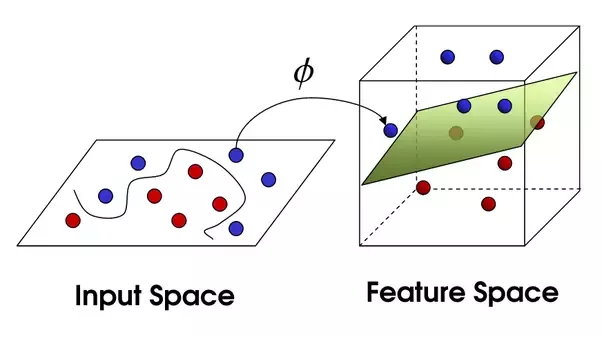
\includegraphics[scale=0.79]{ktr.png}}
\caption{Kernel trick representation}
\end{figure}


\subsection{Pros and Cons associated with SVM} \label{Pros and Cons associated with SVM}

\noindent If we compare, there are quiet a few positives than the negatives of SVM like it is very effective in high dimensional spaces. Even where the number of dimensions is greater than the number of samples it yet has its effect. It uses a subset of training points in the decision function (called support vectors) that makes the memory more efficient. The algotithm is versatile where different Kernel functions can be specified for the decision function. Common kernels are
provided, but it is also possible to specify custom kernels. 

\noindent There are very few negatives, some of them are it does not perform well when we have large data set because the required training time is higher. When the data set is noisy the performance is not good enough, that is the target classes are overlapping and lastly SVM does not directly provide probability estimates, these are calculated using an expensive five-fold cross-validation.


\newpage

\section{k-Nearest Neighbors algorithm (k-NN)} \label{k-Nearest Neighbors algorithm (k-NN)}
\noindent The k-nearest neighbors algorithm (k-NN) is a non-parametric method used for classification and regression. The closest neighbor (NN) rule distinguishes the classification of unknown data point on the basis of its closest neighbor whose class is already known. The value ‘k’ indicates how many nearest neighbors are to be considered to characterize class of a sample data point. It makes utilization of the more than one closest neighbor to determine the class in which the given data point belongs to and consequently it is called as KNN. If k = 1, then the object is simply assigned to the class of that single nearest neighbor.


\begin{figure}[H]
\centering
{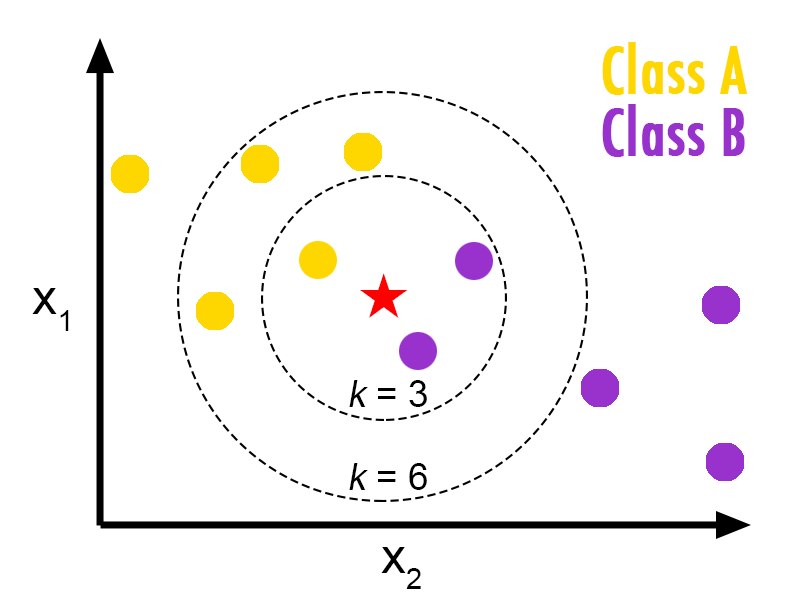
\includegraphics[scale=0.60]{knn.png}}
\caption{Nearest Neighbours for different values of k}
\end{figure}


\subsection{Pros and Cons associated with k-NN} \label{Pros and Cons associated with k-NN}
\noindent Here it is simpler to implement. k-NN employs lazy learning and generalizes during testing which makes it a real time algorithm. It also handles multi-class cases naturally and can do well in practice with enough representative data. 

\noindent On the other hand when the data sets are large, lazy learning requires that most of k-NN's computation be done during testing, rather than during training which increases the computational time. Searching for the nearest neighbour is a time consuming task. The set back over here is inputs can commonly be "close" to many data points. This reduces the effectiveness of k-NN, since the algorithm relies on a correlation between closeness and similarity.

\newpage

\section{Decision tree learning} \label{Decision tree learning}

\noindent Decision tree learning uses a decision tree (as a predictive model) to go from observations about an item (represented in the branches) to conclusions about the item's target value (represented in the leaves). Tree models where the target variable can take a discrete set of values are called classification trees; in these tree structures, leaves represent class labels and branches represent conjunctions of features that lead to those class labels. To predict a response, follow the decisions in the tree from the root (beginning) node down to a leaf node. The leaf node contains the response.


\begin{figure}[H]
\centering
{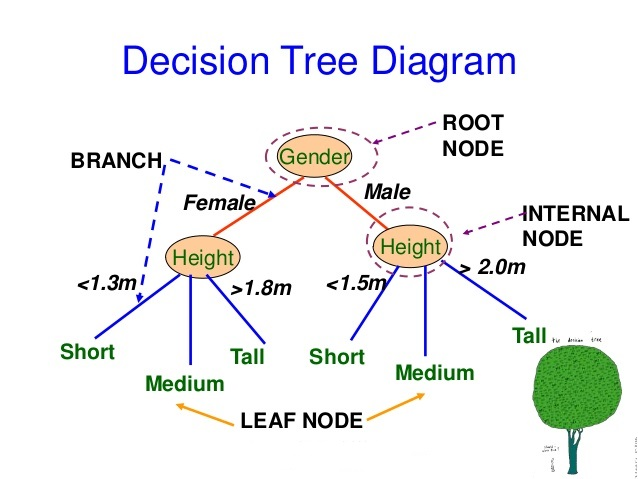
\includegraphics[scale=0.48]{dt.jpg}}
\caption{Decision tree diagram}
\end{figure}

\noindent MATLAB provides 3 types of decision trees depending on the maximum number of splits possible.


\begin{figure}[H]
\centering
{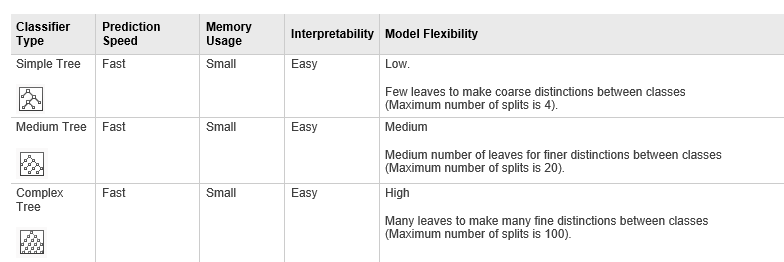
\includegraphics[scale=0.87]{table.png}}
\caption{Types of Decision Trees in MATLAB}
\end{figure}

\newpage
\subsection{Pros and Cons associated with Decision tree} \label{Pros and Cons associated with Decision tree}

\noindent They are very fast to build and test. Another strong behavior is that they work on highly non-linear data, easy to understand, visualise and require minimum assumption. Even the nonlinear relationships between parameters do not affect tree performance.

\noindent Whereas the weekness here is even a small change in input data can at times, cause large changes in the tree. Changing variables, excluding duplication information, or altering the sequence midway can lead to major changes and might possibly require redrawing the tree. Decision Trees do not work well if you have smooth boundaries, that is they work best when you have discontinuous piece wise constant model. If you truly have a linear target function decision trees are not the best. They do not work best if you have a lot of un-correlated variables and a tree with many levels and branches can lead to an over optimized result, or many false positives due to multiple comparison.